\section{Winkelfunktionen}
\begin{minipage}{.5\textwidth}
 \begin{shaded}\begin{align}
\sin{\alpha} &=\frac{a}{c}\\
\cos{\alpha} &=\frac{b}{c}\\
\tan{\alpha} &=\frac{a}{b}\\
\cot{\alpha} &=\frac{b}{a}
\end{align}
\end{shaded}
\end{minipage}\begin{minipage}{.5\textwidth}\begin{center} 
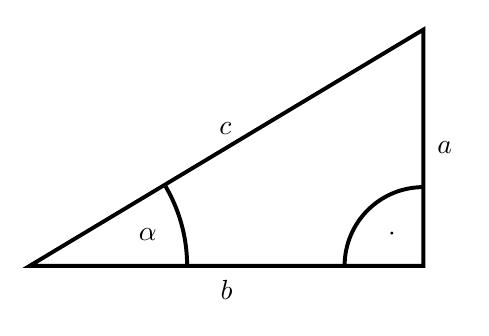
\begin{tikzpicture}[line width=.5mm]
%Dreieck
 \draw (0,0)--++(0:5cm)--++(90:3cm)--cycle;
\draw (2cm,0) arc (0:30.96:2cm);
\draw (4cm,0) arc (180:90:1cm);
%Deschriftung
\draw (4.6cm,.4)node{$\cdot$};
\draw (1.5cm,.4cm)node{$\alpha$};
\draw (5cm,1.5cm)node[right=1pt]{$a$};
\draw (2.5cm,0cm)node[below=1pt]{$b$};
\draw (30.96:2.9cm)node[above=1pt]{$c$};
\end{tikzpicture}
\end{center}
\end{minipage}

\bla{Rechenregeln}
\begin{shaded}
 \begin{align}
  \cos x &=\sin\left(x+\frac{\pi}{2}\right)&   \sin x &=\cos\left(x+\frac{\pi}{2}\right) \\
  \tan x &=\frac{\sin x}{\cos x}=\frac{1}{\cot x}& \cot x &=\frac{\cos x}{\sin x}=\frac{1}{\tan x}
\end{align}
\end{shaded}

\bla{Trigonometrischer Pythagoras}
\begin{shaded}
  \begin{equation}
\sin^2 x+ \cos^2 x =1
  \end{equation}
\end{shaded}

\bla{Addition von Winkeln}
\begin{shaded}
\begin{subequations}
  \begin{equation}
\sin\left(x_1\pm x_2\right)= \sin x_1 \cdot \cos x_2\pm \cos x_1 \cdot \sin x_2
  \end{equation}
  \begin{equation}
\cos\left(x_1\pm x_2\right)= \cos x_1 \cdot \cos x_2\mp \sin x_1 \cdot \sin x_2
  \end{equation}
  \begin{equation}
\tan\left(x_1\pm x_2\right)=\frac{\tan x_1 \pm \tan x_2}{1 \mp \tan x_1 \cdot \tan x_2}
  \end{equation}
  \begin{equation}
\cot\left(x_1\pm x_2\right)=\frac{\cot x_1 \cdot \cot x_2 \mp 1}{\cot x_2 \pm \cot x_1}
  \end{equation}
\end{subequations}
\end{shaded}

\bla{Multiplikation von Winkeln}
\begin{shaded}
\begin{subequations}
  \begin{equation}
\sin x_1 \cdot \sin x_2 =\frac{1}{2}\cdot \left(\cos (x_1 - x_2)- \cos(x_1+x_2)\right)
  \end{equation}
  \begin{equation}
\cos x_1 \cdot \cos x_2 = \frac{1}{2}\cdot \left(\cos(x_1 -x_2)+\cos(x_1+x_2)\right)
  \end{equation}
  \begin{equation}
\sin x_1 \cdot \cos x_2 =\frac{1}{2}\cdot \left(\sin(x_1 -x_2)+ \sin(x_1+x_2)\right)
  \end{equation}
  \begin{equation}
\tan x_1 \cdot \tan x_2 =\frac{\tan x_1 + \tan x_2}{\cot x_1+\cot x_2} 
  \end{equation}
\end{subequations}
\end{shaded}
\bla{Umrechnung Grad- $\Rightarrow$ Bogenmaß}
\begin{shaded}
 \begin{equation}
  x=\frac{\pi}{180^\circ}\cdot\alpha
 \end{equation}
\end{shaded}
\bla{Umrechnung Bogen- $\Rightarrow$ Gradmaß}
\begin{shaded}
 \begin{equation}
  \alpha=\frac{180^\circ}{\pi}\cdot x
 \end{equation}
\end{shaded}